%%%%%%%%%%%%%%%%%%%%%%%%%%%%%%%%%%%%%%%%%
% fphw Assignment
% LaTeX Template
% Version 1.0 (27/04/2019)
%
% This template originates from:
% https://www.LaTeXTemplates.com
%
% Authors:
% Class by Felipe Portales-Oliva (f.portales.oliva@gmail.com) with template 
% content and modifications by Vel (vel@LaTeXTemplates.com)
%
% Template (this file) License:
% CC BY-NC-SA 3.0 (http://creativecommons.org/licenses/by-nc-sa/3.0/)
%
%%%%%%%%%%%%%%%%%%%%%%%%%%%%%%%%%%%%%%%%%

%----------------------------------------------------------------------------------------
%	PACKAGES AND OTHER DOCUMENT CONFIGURATIONS
%----------------------------------------------------------------------------------------

\documentclass[
	12pt, % Default font size, values between 10pt-12pt are allowed
	%letterpaper, % Uncomment for US letter paper size
	%spanish, % Uncomment for Spanish
]{fphw}
\usepackage{subcaption}
% Template-specific packages
\usepackage[utf8]{inputenc} % Required for inputting international characters
\usepackage[T1]{fontenc} % Output font encoding for international characters
\usepackage{mathpazo} % Use the Palatino font
\usepackage{amsmath}
\usepackage{graphicx} % Required for including images
\usepackage{hyperref}
\usepackage{booktabs} % Required for better horizontal rules in tables
\usepackage{listings} % Required for insertion of code
\usepackage{enumerate} % To modify the enumerate environment
\usepackage{bbm}% from mathbbm.sty
%----------------------------------------------------------------------------------------
%	ASSIGNMENT INFORMATION
%----------------------------------------------------------------------------------------

\title{Homework \#2} % Assignment title

\author{Fanyi Meng (223015127)} % Student name

\date{March 31st, 2024} % Due date

\institute{The Chinese University of Hongkong, Shenzhen \\ Computer and Information Engineering} % Institute or school name

\class{Advanced Machine Learning (AIR 6002)} % Course or class name

\professor{Prof Tongxin Li} % Professor or teacher in charge of the assignment

%----------------------------------------------------------------------------------------

\begin{document}
\maketitle % Output the assignment title, created automatically using the information in the custom commands above

%----------------------------------------------------------------------------------------
%	ASSIGNMENT CONTENT
%----------------------------------------------------------------------------------------

\section*{Question 1: Adaboost}
\begin{problem}

	
	\begin{enumerate}[(\itshape a\normalfont)]
		\itemsep0.3em
		\parskip0.3em
		\item  Let $h_t: \mathbb{R}^m \rightarrow\{-1,1\}$ be the weak classifier obtained at step $t$, and let $\alpha_t$ be its weight. Recall that the final classifier is
		$$
		H(x)=\operatorname{sign}(f(x))=\operatorname{sign}\left(\sum_{i=1}^T \alpha_t h_t(x)\right).
		$$
		Suppose $\left\{\left(x_1, y_1\right), \ldots,\left(x_N, y_N\right)\right\} \subset \mathbb{R}^m \times\{-1,1\}$ is our training dataset. Show that the training set error of the final classifier can be bounded from above if an exponential loss function is used:

		$$
		E=\frac{1}{N} \sum_{i=1}^N \exp \left(-y_i f\left(x_i\right)\right) \geq \frac{1}{N} \sum_{i=1}^N \mathbbm{1}\left(H\left(x_i\right) \neq y_i\right)
		$$
		where $\mathbbm{1}$ is the indicator function.
		\item Find $D_{T+1}(i)$ in terms of $Z_t, \alpha_t, x_i, y_i$, and the classifier $h_t$, where $T$ is the last timestep and $t \in\{1, \ldots, T\}$. Recall that $Z_t$ is the normalization factor for distribution $D_{t+1}$: 
		$$
		Z_t=\sum_{i=1}^N D_t(i) \exp \left(-\alpha_t y_i h_t\left(x_i\right)\right).
		$$
		\item Show that $E=\sum_{i=1}^N \frac{1}{N} e^{\sum_{t=1}^T-\alpha_t y_i h_t\left(x_i\right)}.$ 

		\item Show that 
		$$
		E=\prod_{t=1}^T Z_t.
		$$
		\item Show that the normalizer $Z_t$ can be written as 
		$$
		Z_t=\left(1-\epsilon_t\right) \exp \left(-\alpha_t\right)+\epsilon_t \exp \left(\alpha_t\right)
		$$
		where $\epsilon_t$ is the training set error of weak classifier $h_t$ for the weighted dataset:
		$$
		\epsilon_t=\sum_{i=1}^N D_t(i) \mathbbm{1}\left(h_t\left(x_i\right) \neq y_i\right).
		$$
		
	\end{enumerate}
	

\end{problem}
\begin{problem}
	\begin{enumerate}[(\itshape a\normalfont)]
		\setcounter{enumi}{5}
	\item We derived all of this because it is hard to directly minimize the training set error, but we can greedily minimize the upper bound $E$ on this error. Show that choosing $\alpha_t$ greedily to minimize $Z_t$ at each iteration leads to the choices in AdaBoost:  
		$$
		\alpha_t^*=\frac{1}{2} \ln \left(\frac{1-\epsilon_t}{\epsilon_t}\right).
		$$
		\item  \textbf{AIR6002} Implement the \url{GradientBoosting.fit()} and \url{AdaBoost.fit()} methods in the notebook ``Q1\_AdaBoost.ipynb" provided for you. 

Some important notes and guidelines:


		\begin{itemize}
		\item For both methods, make sure to work with the class attributes provided to you. Namely, after \url{GradientBoosting.fit ()} is called, \url{self.clfs} should be appropriately filled with the \url{self.n_clfs} trained weak hypotheses. Similarly, after \url{AdaBoost.fit()} is called, \url{self.clfs} and \url{self.coefs} should be appropriately filled with the \url{self.n_clfs} trained weak hypotheses and their coefficients, respectively.
		\item \url{AdaBoost.fit()} should additionally return an $(N, T)$ shaped numpy array D such that \url{D[:, t]} contains $D_{t+1}$ for each $t \in\{0, \ldots,$ \url{self.n_clfs}$\}$.

		\item For the \url{AdaBoost.fit( )} method, use the 0/1 loss instead of the exponential loss.
		\end{itemize} 



\item \textbf{AIR6002}
Plot the loss curves for gradient boosting and for AdaBoost. 
Describe and explain the behaviour of the two loss curves you plot. You should consider two kinds of behaviours: the smoothness of the curves and the final values that the curves approach. 



\item \textbf{AIR6002} Compare the final loss values of the two models. Which performed better on the classification dataset?
% Solution I: Gradient boosting performed better on training but AdaBoost performed better on test. That is, AdaBoost performed better overall as it is naturally more inclined to a classification dataset (it uses classifiers as opposed to regressors). 



\item \textbf{AIR6002}For AdaBoost, where are the dataset weights the largest, and where are they the smallest? 

Hint: \textit{Watch how the dataset weights change across time in the animation.}

\end{enumerate}
\end{problem}
\section*{Answer \footnote{Some of the Answer 1 were referenced from\url{https://cse.buffalo.edu/~jcorso/t/CSE555/files/lecture_boosting.pdf}}}
\begin{enumerate}[(\itshape a\normalfont)]
	\itemsep0.3em
	\parskip0.3em
	\item 
	
	Since $f(x_i) = \text{sign}(f(x_i))\,|f(x_i)| = H(x_i)\,|f(x_i)| $
	
	
	And:
	\begin{itemize}
	\item If \( H(x_i) \neq y_i \) then $ \mathbbm{1}(H(x_i) \neq y_i) $ \( = 1 \leq \)  \(  e^{|f(x_i)|} \).
	\item If \( H(x_i) = y_i \) then  $ \mathbbm{1}(H(x_i) \neq y_i) $ \( = 0 \leq \)  \(  e^{-|f(x_i)|} \).
	\end{itemize}
	
	So, the inequality holds for each term
	\begin{equation*}
		\mathbbm{1}(H(x_i) \neq y_i) \leq \exp(-y_i f(x_i)) 
	\end{equation*}
	
	and hence, the inequality is true.
	\item \begin{align*}
		D_{T+1}(i) &= \frac{1}{Z_T} D_T(i) \exp(-\alpha_T y_i h_T(x_i))  \\
				   &= \frac{1}{Z_T Z_{T-1}} D_{T-1}(i) \exp \left[ -y_i (\alpha_t h_T(x_i) + \alpha_{t-1} h_{T-1}(x_i)) \right] \\
				   &= \cdots \\
				   &= \frac{1}{Z_1 \cdots Z_T} D_1(i) \exp \left[ -y_i (\alpha_T h_T(x_i) + \cdots + \alpha_1 h_1(x_i)) \right] \\
				   &= \prod_1^{T}\frac{1}{Z_t}\exp \left( -y_i \sum_{1}^{T}\alpha_t h_t\left(x_i\right)\right).	
				\end{align*}
	\item $E=\frac{1}{N} \sum_{i=1}^N \exp \left(-y_i f\left(x_i\right)\right)	$, so $E=\sum_{i=1}^N \frac{1}{N} e^{\sum_{t=1}^T-\alpha_t y_i h_t\left(x_i\right)}.$
	\item Following (b), we also have $\sum_i^N D_{T+1}(i) = 1$, so 
	\begin{equation*}
		\sum_{i=1}^{n} D_t(x_i) = \prod_1^{T}\frac{1}{Z_t} \sum_{i=1}^{N} \frac{1}{N}\exp[-y_i f(x_i)] = 1 
	\end{equation*}
	implies:
	\begin{equation*}
		\prod_{t=1}^T Z_t=\frac{1}{N} \sum_{i=1}^N \exp \left(-y_i f\left(x_i\right)\right)=E. 
	\end{equation*}
	
	\item The equation can be represented as :
	\begin{equation*}
		Z_t = \sum_{i}^{N} D_t(x_i) \exp [-y_i \alpha_t h_t(x_i)](\mathbbm{1}\left(h_t\left(x_i\right) = y_i\right)+\mathbbm{1}\left(h_t\left(x_i\right) \neq y_i\right))
	\end{equation*}
	As $y_i h_t(x_i) =1 $ when $h_t\left(x_i\right) = y_i$ and $y_i h_t(x_i) =-1 $ otherwise, so:
	\begin{align*}
		Z_t = &\sum_{i}^N D_t(i) \exp [-\alpha_t] \mathbbm{1}\left(h_t\left(x_i\right) = y_i\right) + \sum_{i}^N D_t(i) \exp [\alpha_t] \mathbbm{1}\left(h_t\left(x_i\right) \neq y_i\right)\\
			= &\left(1-\epsilon_t\right) \exp \left(-\alpha_t\right)+\epsilon_t \exp \left(\alpha_t\right)
	\end{align*}
	

	\item By calculating the gradient of (e):, we get:
	\begin{equation*}
		\left(\epsilon_t-1\right) \exp \left(-\alpha_t\right)+\epsilon_t \exp \left(\alpha_t\right) = 0
	\end{equation*}
	which implies: 
	\begin{equation*}
		\exp \left(\alpha_t\right) = \sqrt{\frac{1-\epsilon_t}{\epsilon_t}} 
	\end{equation*}
	so $$
	\alpha_t^*=\frac{1}{2} \ln \left(\frac{1-\epsilon_t}{\epsilon_t}\right).
	$$
	\item The code can be viewed in the code part.
	\item Gradient Boosting seems to be more smooth and has a good performance on training dataset, but something like overfitting probably occurs since the test loss grows as the n clfs grows.
	Adaboost is not smooth but has a better performance on test dataset.
	\item Adaboost. 
	\item For the data which is predicted wrong in the origin model, the weights are larger. And for the data which has been predicted to be true, the weights are smaller.
	
	\begin{figure}[h!]
		\centering
		\begin{subfigure}[b]{0.45\textwidth}
		  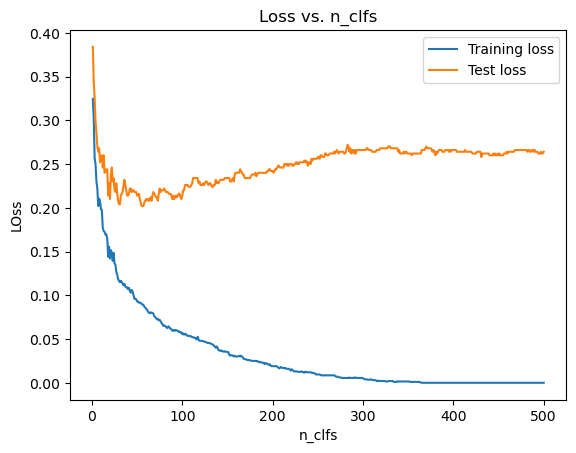
\includegraphics[width=\textwidth]{GB_loss.png}
		  \caption{Gradient boosting Loss}
		  \label{fig:sub1}
		\end{subfigure}
		\hfill
		\begin{subfigure}[b]{0.45\textwidth}
		  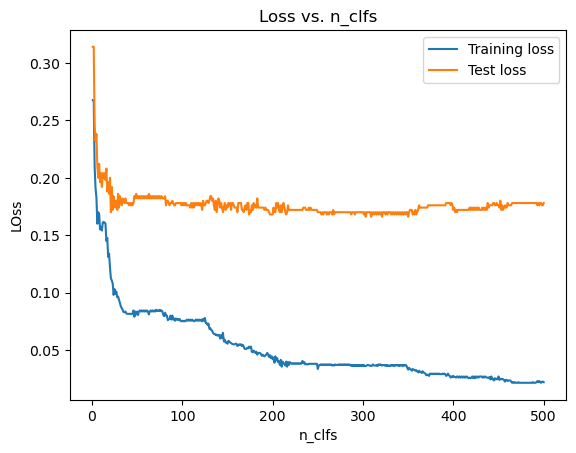
\includegraphics[width=\textwidth]{AB_loss.png}
		  \caption{Adaboost Loss}
		  \label{fig:sub2}
		\end{subfigure}
		\caption{Loss curves for gradient boosting and for AdaBoost}
		\label{fig:images}
	  \end{figure}
\end{enumerate}

%------------------------------------------------
%----------------------------------------------------------------------------------------

\section*{Question 2: Recommendation Systems}

\begin{problem}
	\begin{enumerate}[(\itshape a\normalfont)]
	\itemsep0.3em
	\parskip0.3em
	\item What are the differences between collaborative filtering and content-based methods? 
    


    \item Suppose we have $m$ items and $n$ users. Let $\Omega$ be the set of indices of observed ratings given by the users on the items. Provide the objective function of content-based recommendation for users, where the model class is a neural network with two hidden layers. You need to define the notations clearly. In addition, explain how to make recommendations for a new user using your model. 
\end{enumerate}
  
	


\end{problem}

%------------------------------------------------
\section*{Answer}
\begin{enumerate}[(\itshape a\normalfont)]
\item Collaborative filtering  relies on the user-itsm interaction. It makes recommendations based on patterns of users' behavior with items, without requiring knowledge about the items themselves. Content-Based Methods focus on the properties of the items. Recommendations are made by analyzing the content of the items and the profile of the user's preferences. So Collaborative Filtering can provide more personalized recommendations and Content-Based  Methods  recommend items that are similar to what the user has liked before.
\item \begin{table}[h]
	\centering
	\begin{tabular}{|c|l|}
	\hline
	\textbf{Notations} & \textbf{Description} \\
	\hline
	\( W^{(1)} \) & Weights of the first hidden layer \\
	\( b^{(1)} \) & Biases of the first hidden layer \\
	\( W^{(2)} \) & Weights of the second hidden layer \\
	\( b^{(2)} \) & Biases of the second hidden layer \\
	\( W^{(3)} \) & Weights of the output layer \\
	\( b^{(3)} \) & Bias of the output layer \\
	\( r_{ui} \)  & The element of the rating matrix \\
	\( f_i \)  & The activation function of corresponding layer(e.g. ReLu) \\
	\hline
	
	\end{tabular}
	\caption{notations}
	\label{tab:parameters}
	\end{table}
	Then the objective function can be represented as:
	
\begin{equation}
	J(W^{(1)}, b^{(1)}, W^{(2)}, b^{(2)}, W^{(3)}, b^{(3)}) = \frac{1}{|\Omega|} \sum_{(u,i)\in\Omega} (r_{ui} - \hat{r}_{ui})^2
	\end{equation}
	
	where the predicted rating \( \hat{r}_{ui} \) is computed as:
	
	\begin{equation}
	\hat{r}_{ui} = W^{(3)} f_2\left(W^{(2)} f_1\left(W^{(1)} Z_i + b^{(1)}\right) + b^{(2)}\right) + b^{(3)}
	\end{equation}

	To make recommendations for a new user, we need to collect some user's preferences and use the model to get $r_ui$. By sorting the score, we will recommend the top items.

\end{enumerate}
%----------------------------------------------------------------------------------------
\section*{Question 3:Spectral Clustering}

\begin{problem}
	Prove $\frac{\mathbf{u}^{\top} \mathbf{L u}}{\mathbf{u}^{\top} \mathbf{D u}}=\operatorname{Ncut}(A, B)$. See the definitions on page 23 of Lecture 05-I.
\end{problem}
\section*{Answer}
Since \[ L = D - W \]
and
\[ D = \text{diag}(d_1, \ldots, d_N) \]

And 
\[ u_i = 
\begin{cases} 
\frac{1}{\sqrt{\text{vol}(A)}} & \text{if } i \in A \\
-\frac{1}{\sqrt{\text{vol}(B)}} & \text{if } i \in B
\end{cases} \]

Then, we can express $\mathbf{u}^T L \mathbf{u}$ and $\mathbf{u}^T D \mathbf{u}$ as follows:

\[ \mathbf{u}^T L \mathbf{u} = \frac{1}{2} \sum_{i,j} w_{ij}(u_i - u_j)^2 = \sum_{i \in A, j \in B} w_{ij} \left( \frac{1}{\sqrt{\text{vol}(A)}} + \frac{1}{\sqrt{\text{vol}(B)}} \right)^2 \]

\[ \mathbf{u}^T D \mathbf{u} = \sum_{i} d_i u_i^2 = \sum_{i \in A} \frac{d_i}{\text{vol}(A)^2} + \sum_{j \in B} \frac{d_j}{\text{vol}(B)^2} =\frac{1}{\text{vol}(A)} +\frac{1}{\text{vol}(B)} \]

Because the sums of the degrees for vertices in each set $A$ and $B$ equal the volume of those sets, respectively.

Therefore, the normalized cut (Ncut) for the partition of the graph into sets $A$ and $B$ is given by:

\[ \text{Ncut}(A, B) = \frac{\mathbf{u}^T L \mathbf{u}}{\mathbf{u}^T D \mathbf{u}} = \sum_{i \in A, j \in B} w_{ij} \left( \frac{1}{\text{vol}(A)} + \frac{1}{\text{vol}(B)} \right) \]

This concludes the proof that the expression $\frac{\mathbf{u}^T L \mathbf{u}}{\mathbf{u}^T D \mathbf{u}}$ is equal to the normalized cut value.

%------------------------------------------------

\section*{Question 4:Semi-supervised Learning }

\begin{problem}
	\begin{enumerate}[(\itshape a\normalfont)]
	\item
    Suppose $\mathbf{x}\in\mathbb{R}^d$ and $\mathbf{y}\in\mathbb{R}^k$ and the training data are $\{(\mathbf{x}_i,\mathbf{y}_i)\}_{i=1}^l\bigcup\{\mathbf{x}_i\}_{i=l+1}^n$. Let $\mathbf{A}\in\mathbb{R}^{n\times n}$ be an affinity matrix constructed from the training data. 
	\begin{enumerate}[i)]
	\item Show the objective function of linear regression with square loss and graph regularization. For simplicity, do not consider the bias term. 
	\item Compute the gradient of the objective function with respect to the parameters. 
	\item Is there a closed-form solution? If yes, find it.
\end{enumerate}
    \item In the label propagation algorithm, why do we need to use $\mathbf{D}^{-1}\mathbf{W}$ instead of $\mathbf{W}$? Why do we set $\hat{\mathbf{Y}}_l^{(t+1)} \leftarrow \mathbf{Y}_l$? If there are more than 2 classes, how do we set $\mathbf{Y}^{(0)}$? 
\end{enumerate}
\end{problem}
\section*{Answer}
\begin{enumerate}[(\itshape a\normalfont)]
	\item\begin{enumerate}[i)]
	\item 
\[ J(w) = \frac{1}{2} \sum_{i=1}^l (y_i - w^T x_i)^2 + \frac{\lambda}{2} w^T (D-A) w \](D is the degree matrix of the graph)
\item The gradient is: \[ \nabla_w J(w) = \sum_{i=1}^l (w^T x_i - y_i) x_i + \lambda (D-A) w \]
\item The closed form is: \[ w = (X^T X + \lambda (D-A))^{-1} X^T Y \]
\end{enumerate}
\item \begin{enumerate}[i)]
	\item Since the degree matrix D contains the information of the degree, so using $\mathbf{D}^{-1}\mathbf{W}$ will make each data sample have the same impact on its neighbor.
	\item Since we want to keep the same label for the labeled data.
	\item One-hot Encoding is one possible method.
\end{enumerate}
\end{enumerate}
\section*{Question 5: Graph Neural Networks}

\begin{problem}
\begin{enumerate}[(\itshape a\normalfont)]
	\item In GNN, given $\hat{\mathbf{A}}$, how to compute $\hat{\mathbf{A}}^c:=\underbrace{\hat{\mathbf{A}}\hat{\mathbf{A}}\cdots \hat{\mathbf{A}}}_c$ efficiently when $c$ is large? 
    
    \item Show the loss functions of node classification, graph classification, and link prediction. Explain your notations.
    
    \item Provide two examples of algorithms for each learning types or methods:
    \begin{itemize}
        \item parametric method
        \item nonparametric method
        \item inductive learning
        \item transductive learning
        \item semi-supervised learning
    \end{itemize}
\end{enumerate}

\end{problem}

\section*{Answer}
\begin{enumerate}[(\itshape a\normalfont)]
\item Since $\hat{\mathbf{A}}$ is always invertible, we can calculate the EVD of the matrix as $\hat{\mathbf{A}}$ = $\mathbf{U} \Lambda \mathbf{U}^{-1}$, so $\hat{\mathbf{A}}^c = \mathbf{U} \Lambda^C \mathbf{U}^{-1}$
\item Here is the notation.\footnote{Some of this answer were referenced from\url{https://www.cs.mcgill.ca/~wlh/grl_book/files/GRL_Book-Chapter_6-GNNs_in_Practice.pdf}}

$\begin{array}{|c|l|}
	\hline
	\textbf{Notation} & \textbf{Description} \\
	\hline
	V_{\text{train}} & \text{Set of nodes used for training.} \\
	\hline
	z_u & \text{Embedding of node u.} \\
	\hline
	y_u & \text{Class label of node u .} \\
	\hline
	T & \text{Set of graphs used for training.} \\
	\hline
	z_{G_i} & \text{Graph-level embedding of graph } G_i. \\
	\hline
	y_{G_i} & \text{Target value for training graph } G_i  \\
	\hline
	E & \text{Set of edges, representing all possible node pairs.} \\
	\hline
	y_{uv} & \text{Actual label indicating whether a link exists between node pair } (u, v). \\
	\hline
	\hat{y}_{uv} & \text{Predicted probability that a link exists between node pair } (u, v). \\

	\hline
	
	\end{array}
$	

Loss function for node classification: 
\begin{equation*}
	L = -\sum_{u \in V_{\text{train}}} \log(\text{softmax}(z_u)[y_u])
\end{equation*}
Loss function for graph classification:
\begin{equation*}
	L = -\sum_{G_i \in T} \log(\text{softmax}(z_{G_i})[y_{G_i}])
\end{equation*}	
Loss function for link prediction:
\begin{equation*}
L = -\sum_{(u, v) \in E} y_{uv} \log(\hat{y}_{uv}) + (1 - y_{uv}) \log(1 - \hat{y}_{uv})
\end{equation*}	
\newpage
\item\textbf{Parametric method}:Linear Regression, Logistic Regression

\textbf{Nonparametric method }:K-Nearest Neighbors,Decision Trees

\textbf{Inductive Learning}:Support Vector Machines,Random Forest

\textbf{Transductive Learning}:Label Propagation,Label Spreading

\textbf{Semi-supervised Learning}:Autoencoders,Semi-Supervised SVM
\end{enumerate}


\section*{Question 6: Nonlinear Dimensionality Reduction}

\begin{problem}
	\begin{enumerate}[(\itshape a\normalfont)]
	\item Show the algorithm of multidimensional scaling here. 
    
    \item Present a method for out-of-sample extension of t-SNE. In other words, reduce the dimension of new samples using the training result of t-SNE. 
    
    \item Given a dataset, suppose most of the samples are normal or good data, and there are a few outliers. Design a method or strategy to detect these outliers bassed on the methods learned in Lecture 07.
\end{enumerate}
\end{problem}
\section*{Answer}
\begin{enumerate}[(\itshape a\normalfont)]
\item \begin{enumerate}[$\bullet$]
\item  Calculate the distance between the datas.(e.g.Euclidean distance)
\item  Build Gram matrix $B$ , where \[
	b_{ij} = -\frac{1}{2}(d_{ij}^2 - \bar{d}_{i\cdot}^2 - \bar{d}_{\cdot j}^2 + \bar{d}_{\cdot\cdot}^2)
	\]
\item Calculate EVD of $B$,so \[
	B = V \Lambda V^T
	\]
\item Choose the eigen vector for the top $k$ eigenvectors, then get the low dimension \[
	X = V_k \sqrt{\Lambda_k}
	\]
\end{enumerate}
\item Firstly, we can use t-SNE to map it into low dimension. And then we find its neighbors and calculate the center of there neighbors as the new sample.
\item We can use Non-Linear Dimensionality Reduction to map it into low dimension and find whetehr the data has enough neighbors. Outliers may has no neighbor.

\end{enumerate}

\section*{Question 7: Generative Models}

\begin{problem}
	\begin{enumerate}[(\itshape a\normalfont)]
	\item Derive the evidence lower bound (ELBO) for the VAE model. 

    \item Derive the objective functions for the generator and discriminator in a GAN, respectively. 
    

    \item Briefly explain the relationship between diffusion models and Langevin dynamics.  
\end{enumerate}
\end{problem}
\section*{Answer}
\begin{enumerate}[(\itshape a\normalfont)]
\item	\[ \text{ELBO} = \mathbb{E}_{\mathbf{z}\sim q_{\phi}(\mathbf{z};\mathbf{x})}[\log p_{\theta}(\mathbf{x}|\mathbf{z})]-D_{KL}(q_{\phi}(\mathbf{z}|\mathbf{x})||p(\mathbf{z})) \]
Where:

- $p{\theta}(x|z)$ is the likelihood of observing data $x$ given latent variables $z$.

- $q{\phi}(z|x)$ is the variational distribution (encoder) that approximates the true posterior distribution of latent variables given data.

- $p(z)$ is the prior distribution of latent variables.

- $\text{KL}(q{\phi}(z|x)||p{\theta}(z))$ is the Kullback-Leibler (KL) divergence between the variational distribution and the prior.

\item Generator's objective:
\[ \min_G \max_D V(D, G) = \mathbb{E}_{x \sim p_{\text{data}}(x)}[\log D(x)] + \mathbb{E}_{z \sim p(z)}[\log(1 - D(G(z)))] \]

Discriminator's objective:
\[ \min_D \max_G V(D, G) = \mathbb{E}_{x \sim p_{\text{data}}(x)}[\log D(x)] + \mathbb{E}_{z \sim p(z)}[\log(1 - D(G(z)))] \]

Where:

- $p_{\text{data}}(x)$ is the true data distribution.

- $p(z)$ is the prior distribution of noise variables $z$.

- $G(z)$ is the generated data sample.

- $D(x)$ represents the discriminator's output indicating the probability that $x$ is a real data sample.

\item- \textbf{Diffusion models} describe the evolution of a stochastic process over time, where the process starts from an initial distribution and evolves according to a diffusion process. 

- \textbf{Langevin dynamics},  is a type of stochastic differential equation that describes the motion of particles subjected to random forces. In the context of probabilistic modeling, Langevin dynamics can be used for sampling from probability distributions by simulating the motion of particles according to the gradients of the log-probability density.
\end{enumerate}
\section*{Question 8: Graph Convolutional Network}

\begin{problem}
	\begin{enumerate}[(\itshape a\normalfont)]
		\item \textbf{AIR6002} Implement the \url{GCNLayer.forward()} in the notebook ``Q8\_GCN.ipynb" provided for you. 
	
		\item \textbf{AIR6002} Define the adjacency matrix of the graph in the notebook with self-connections.  

	
		\item \textbf{AIR6002} Apply the GCN layer defined in (1) on the graph in (2), and write down the output features for all nodes. 
	\end{enumerate}
\end{problem}
\section*{Answer}

All these parts are shown in code part.




%------------------------------------------------




%----------------------------------------------------------------------------------------

\end{document}
